
%(BEGIN_QUESTION)
% Copyright 2006, Tony R. Kuphaldt, released under the Creative Commons Attribution License (v 1.0)
% This means you may do almost anything with this work of mine, so long as you give me proper credit

Vannivået i damptrommelen på en kjele måles vanligvis med en differansetrykktransmitter med balanserør til toppen av trommelen for å utligne statisk trykk:

$$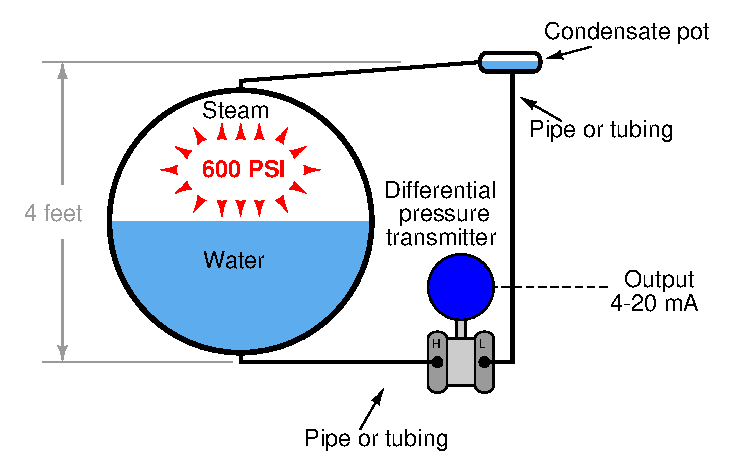
\includegraphics[width=15.5cm]{i00307x01.eps}$$

Siden en damptrommel på 600 PSI går ved høy temperatur, og transmitterens balanserør til trommeltoppen er kaldere enn trommelen, vil damp kondensere til vann i røret, som fylles helt og blir et {\it ``wet leg''}.

Avgjør om statisk damptrykk på 600 PSI krever spesiell kalibrering av transmitteren.

Beskriv hvordan nivåtransmitteren må kalibreres annerledes enn ved tørt kompenseringsben (ingen kondensat), og forklar også hensikten med kondensatpotten.

\underbar{file i00307}
%(END_QUESTION)





%(BEGIN_ANSWER)

Tilstedeværelse av wet leg vil løfte nullpunktet i transmitterområdet med 48" W.C.

\vskip 10pt

De fleste DP-transmittere får {\it noe} kalibreringsfeil ved høye statiske trykk, men dette er vanligvis neglisjerbart.  Transmitteren kan derfor kalibreres normalt på benk med inches WC lufttrykk, uten spesialoppsett.

\vskip 10pt

Det er vanlig å montere en ``kondensatpott'' i toppen av dette vertikale røret for å sikre tilstrekkelig kondensatvolum i wet leg.  Dette reduserer midlertidige kalibreringsfeil som kan oppstå ved tap av kondensat under vedlikeholdsdrenering.

%(END_ANSWER)





%(BEGIN_NOTES)


%INDEX% Measurement, level: condensate pot on wet leg of steam drum level transmitter
%INDEX% Measurement, level: steam drum (wet leg)

%(END_NOTES)
